\documentclass{article}
\usepackage{lmodern}
\usepackage[T1]{fontenc}
\usepackage{shapepar}
\usepackage{microtype}
\usepackage{lipsum}
\usepackage{pgfplots}
\pgfplotsset{compat=1.9}
\usepackage{tikz}
\usetikzlibrary{calc,fit,intersections,folding}
\usepackage{pstricks-add}
\usetikzlibrary{arrows.meta,angles,arrows,quotes,backgrounds}


\begin{document}
\thispagestyle{empty}
\begin{center}
    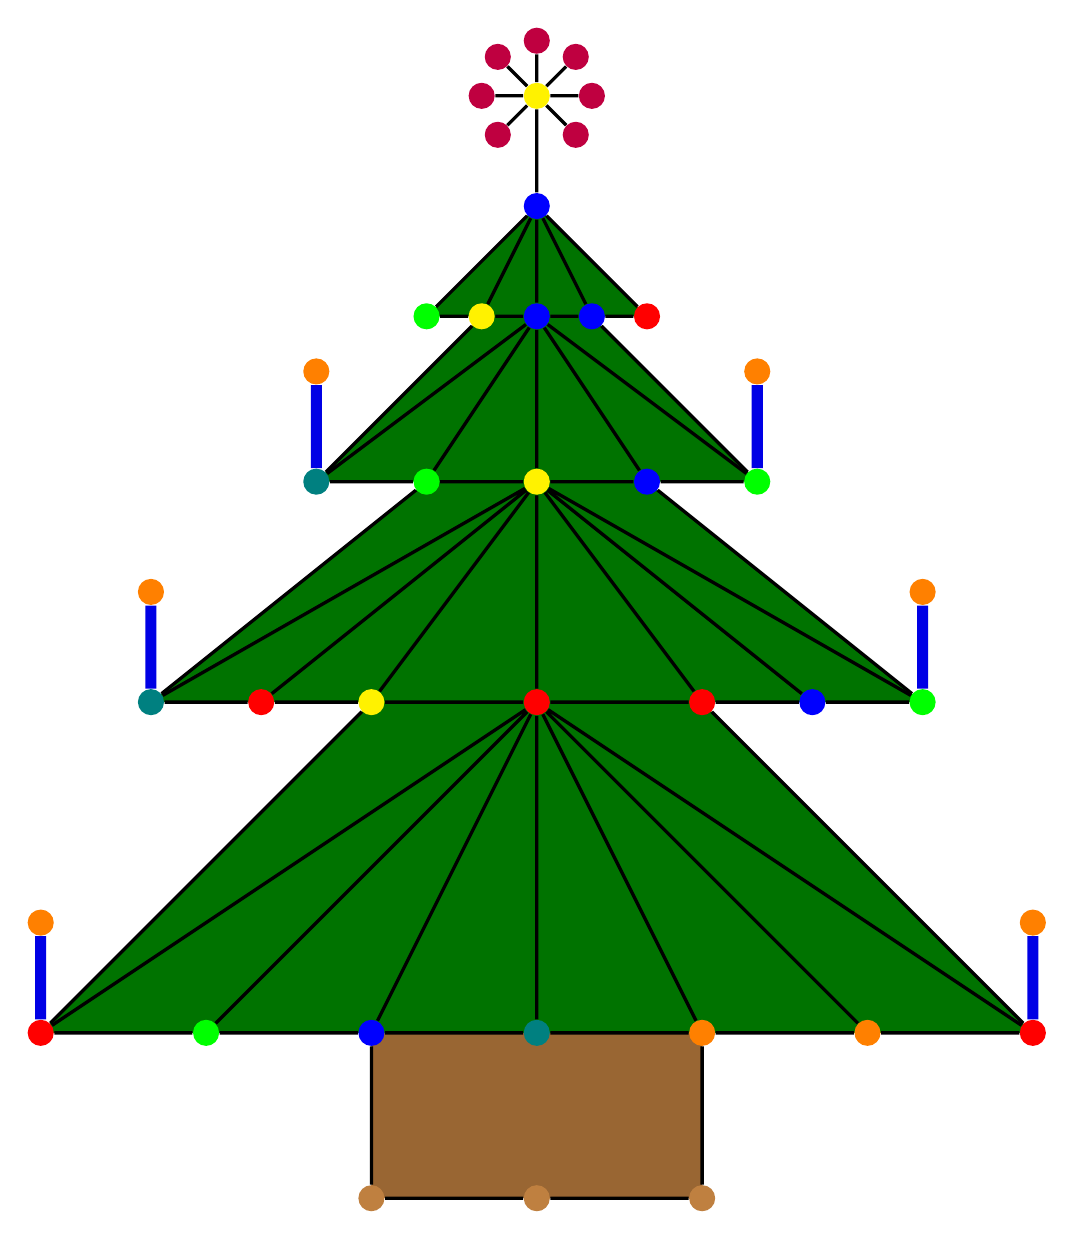
\begin{tikzpicture}[scale = 0.7]
        \node[fill, circle, yellow] (1) at (0,0) {};
        \node[fill, circle, purple] (2) at (-45:1cm) {};
        \node[fill, circle, purple] (3) at (0:1cm) {};
        \node[fill, circle, purple] (4) at (45:1cm) {};
        \node[fill, circle, purple] (5) at (90:1cm) {};
        \node[fill, circle, purple] (6) at (135:1cm) {};
        \node[fill, circle, purple] (7) at (180:1cm) {};
        \node[fill, circle, purple] (8) at (225:1cm) {};
        \node[fill, circle, blue] (9) at (0,-2) {};
        
        \node[fill, circle, green] (10) at (-2,-4) {};
        \node[fill, circle, yellow] (11) at (-1,-4) {};
        \node[fill, circle, blue] (12) at (0,-4) {};
        \node[fill, circle, blue] (13) at (1,-4) {};
        \node[fill, circle, red] (14) at (2,-4) {};

        \node[fill, circle, orange] (15) at (-4,-5) {};
        \node[fill, circle, orange] (16) at (4,-5) {};

        \node[fill, circle, teal] (17) at (-4,-7) {};
        \node[fill, circle, green] (18) at (-2,-7) {};
        \node[fill, circle, yellow] (19) at (0,-7) {};
        \node[fill, circle, blue] (20) at (2,-7) {};
        \node[fill, circle, green] (21) at (4,-7) {};

        \node[fill, circle, orange] (22) at (-7,-9) {};
        \node[fill, circle, orange] (23) at (7,-9) {};

        \node[fill, circle, teal] (24) at (-7,-11) {};
        \node[fill, circle, red] (25) at (-5,-11) {};
        \node[fill, circle, yellow] (26) at (-3,-11) {};
        \node[fill, circle, red] (27) at (-0,-11) {};
        \node[fill, circle, red] (28) at (3,-11) {};
        \node[fill, circle, blue] (29) at (5,-11) {};
        \node[fill, circle, green] (30) at (7,-11) {};

        \node[fill, circle, orange] (31) at (-9,-15) {};
        \node[fill, circle, orange] (32) at (9,-15) {};

        \node[fill, circle, red] (33) at (-9,-17) {};
        \node[fill, circle, green] (34) at (-6,-17) {};
        \node[fill, circle, blue] (35) at (-3,-17) {};
        \node[fill, circle, teal] (36) at (0,-17) {};
        \node[fill, circle, orange] (37) at (3,-17) {};
        \node[fill, circle, orange] (38) at (6,-17) {};
        \node[fill, circle, red] (39) at (9,-17) {};

        \node[fill, circle, brown] (40) at (-3,-20) {};
        \node[fill, circle, brown] (41) at (0,-20) {};
        \node[fill, circle, brown] (42) at (3,-20) {};

        \draw[very thick][very thick] (1) -- (2) (1) -- (3) (1) -- (4) (1) -- (5) (1) -- (6) (1) -- (7) (1) -- (8) (1) -- (9);
        \draw[very thick] (9) -- (10) (9) -- (11) (9) -- (12) (9) -- (13) (9) -- (14);
        \draw[very thick] (10) -- (11) -- (12) -- (13) -- (14);
        \draw[very thick] (12) -- (17) (12) -- (18) (12) -- (19) (12) -- (20) (12) -- (21);
        \draw[line width = 4pt, black!10!blue] (17) -- (15) (21) -- (16);
        \draw[very thick] (17) -- (18) -- (19) -- (20) -- (21);
        \draw[very thick] (17) -- (11) (21) -- (13);

        \draw[very thick] (19) -- (24) (19) -- (25) (19) -- (26) (19) -- (27) (19) -- (28) (19) -- (29) (19) -- (30);
        \draw[line width = 4pt, black!10!blue] (24) -- (22) (30) -- (23);
        \draw[very thick] (24) -- (25) -- (26) -- (27) -- (28) -- (29) -- (30);
        \draw[very thick] (24) -- (18) (30) -- (20);

        \draw[very thick] (27) -- (33) (27) -- (34) (27) -- (35) (27) -- (36) (27) -- (37) (27) -- (38) (27) -- (39);
        \draw[very thick] (33) -- (34) -- (35) -- (36) -- (37) -- (38) -- (39);
        \draw[line width = 4pt, black!10!blue] (33) -- (31) (39) -- (32);
        \draw[very thick] (33) -- (26) (39) -- (28);

        \draw[very thick] (35) -- (40) -- (41) -- (42) -- (37);

    \begin{scope}[on background layer]
        \fill[black!20!brown] (35.center) -- (40.center) -- (42.center) -- (37.center) -- (35.center);
    \end{scope}

    \begin{scope}[on background layer]
        \fill [black!55!green] (9.center) -- (10.center) -- (11.center) -- (17.center) -- (18.center) -- (24.center) -- (26.center) -- (33.center) -- (39.center) -- (28.center) -- (30.center) -- (20.center) -- (21.center) -- (13.center) -- (14.center) -- (9.center);
    \end{scope}

    
    \end{tikzpicture}
\end{center}
\end{document}